%!TEX encoding=UTF-8 Unicode
\chapter{Case Study}
\label{chap:perf}

Optimizing a computational kernel is a complex task, it requires a deep understanding of both the algorithm mechanics and the machine that will execute it.
Simple computational kernels such as matrix multiplication or Cholesky factorization have been subject of years of optimizations, yet some scientists still manage to find improvements.
The task is even more complex when it comes to optimizing a whole actual application, we first need to identify hotspots which means understand where and why the performances are suboptimal.
Once the hotspots are identified, we have to understand their nature and their localization both in terms of code and data structure (if they are memory related).
Finally, when optimizing a real life application, it is important to make the optimizations as clear as possible as not all developers are specialized in \gls{HPC}.

\gls{SOFA}~\cite{Allard07SOFA} is a simulation framework designed for exact interactive simulation.
Indeed, it aims at assisting surgeons with real time simulation thus  it cannot afford to reduce the amount of computation by relying on approximations.
Thus improving \gls{SOFA} performance is crucial, yet most of the developers are not from the \gls{HPC} field.
Our goal is to guide the developers in the optimization process, therefore we need to analyze the  performances of \gls{SOFA} and identify precisely the hotspots.

In this chapter, we present a case study on the performance optimisation of \gls{SOFA}.
It is organized as follow: first we present \gls{SOFA}, its specificities and previous attempt to parallelize or optimize it in \sect{motivations}.
Then, we discuss the existing profiling tools that can be used to analyze the performances of application in \sect{prof-tools}.
After that we detail our experimental methodology and discuss reproducibility matters in \sect{expe-methodo}.
Finally we present our analysis and first conclusions in \sect{sofa-analysis}.

\section{Motivations}
\label{sec:motivations}

Several efforts were made to parallelize the different part of \gls{SOFA}, using its specificities.
Before discussing these efforts, we need to present more precisely the \gls{SOFA} framework.

\subsection{SOFA: a physical simulation framework}

\begin{figure}[htb]
    \centering
    %!TEX encoding=UTF-8 Unicode

\definecolor{StepCol}{HTML}{4575B4}
\definecolor{ObjACol}{HTML}{FDB863}
\definecolor{ObjAICol}{HTML}{FEE090}
\definecolor{ObjBCol}{HTML}{5E3C99}
\definecolor{ObjBICol}{HTML}{B2ADB2}
\definecolor{ForceCol}{HTML}{ED4049}


\tikzset{
  rounded box/.style={
    shape = rectangle,
    draw,
    rounded corners,
    },
  drawed box/.style ={
    rounded box,
    inner sep=.5em,
    draw = #1,
    },
  ObjA-render/.style ={
      circle,
      shading=ball,
      ball color=ObjACol!80!ObjAICol,
      minimum width=1cm,
  },
  ObjA/.style ={
      circle,
      fill=ObjACol,
      minimum width=1cm,
  },
  ObjB/.style ={
      regular polygon,
      regular polygon sides=8,
      fill=ObjBCol,
      minimum width=1cm,
      minimum height=1cm,
  },
  ObjB-render/.style ={
      regular polygon,
      regular polygon sides=8,
      shading=ball,
      ball color=ObjBCol!80!ObjBICol,
      minimum width=1cm,
      minimum height=1cm,
  },
}

\tikzstyle{StepBox} = [drawed box=StepCol]
\tikzstyle{StepA} = [-latex,StepCol,thick]
\tikzstyle{Force} = [-latex,ForceCol,very thick]

\begin{tikzpicture}[scale=0.74,font=\small]


    \node[ObjA] (Ai) at (0,0) {};
    \node[ObjB] (Bi) at (2,0) {};

    \node[StepBox,fit=(Ai) (Bi)] (init) {};

    \node[StepCol,text width=5em] (inittxt) at (0,1.5) {Initial\\State};

    \node[ObjA] (AI) at (4.5,0) {};
    \node[ObjB] (BI) at (5.5,0) {};

    \node[StepBox,fit=(AI) (BI)] (inte) {};


    \node[ObjA] (Ac) at (8,0) {};
    \node[ObjB] (Bc) at (9.5,0) {};

    \node[StepBox,fit=(Ac) (Bc)] (col) {};

    \node[ObjA-render] (Ad) at (12,0) {};
    \node[ObjB-render] (Bd) at (13.5,0) {};

    \node[StepBox,fit=(Ad) (Bd)] (dis) {};


    % Steps

    \draw[StepA] (init.east) -- node[text width=5em,above=2em]
        {Time\\Integration} (inte.west);

    \draw[StepA] (inte.east) --  node[text width=9em,above=2em]
    {Collision detection\\and response}(col.west) {};

    \draw[StepA] (col.east) -- node[text width=5em,above=2em]
        {Rendering} (dis.west) {};

    \path[StepA] (dis.south) edge[out=-160,in=-20] (init.south) {};

    % Forces

    \draw[Force] (Ai.center) -- ++(.8,0) {};
    \draw[Force] (Bi.center) -- ++(-.8,0) {};

    \draw[Force] (Ac.east) -- ++(-.4,0) {};
    \draw[Force] (Bc.west) -- ++(.4,0) {};


\end{tikzpicture}
% vim: et si sta lbr  sw=4 ts=4 spelllang=en_us

    \caption[The simulation loop]{The simulation loop}
    \label{fig:simu-pipeline}
\end{figure}

In \gls{SOFA}, simulation can be seen as a loop depicted in \fig{simu-pipeline}: we start from an initial configuration were a set of objects are subject to a force field.
Then we have to solve a system of equation to compute the next position of each object.
The third step consist in detecting overlap between objects and applying repulsing force to simulate the collision.
Finally the result of these step is displayed (rendered) and we are back the beginning.
The time integration and the collisions detection are the most costly steps.
Hence many algorithms  were developed to compute these steps efficiently each algorithm being more appropriate for simulating one type of object.

\begin{figure}[htb]
    \centering
    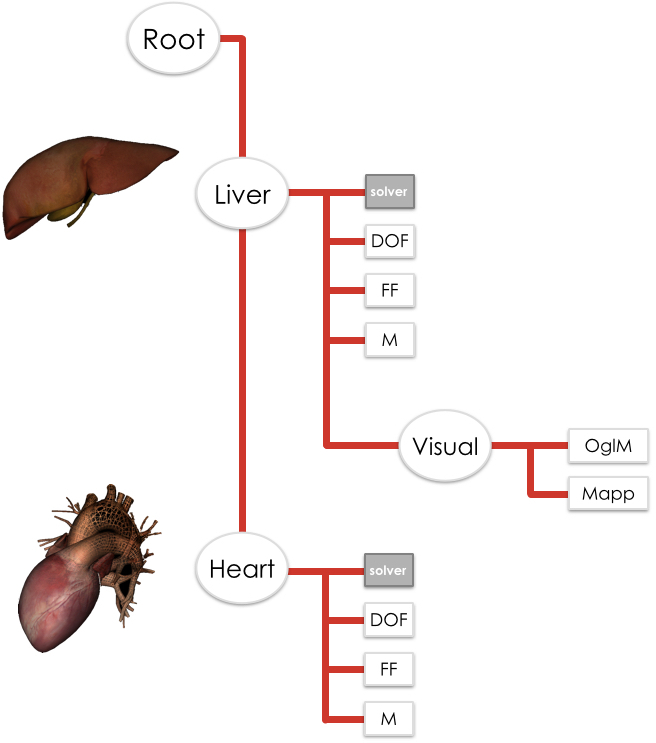
\includegraphics[width=\textwidth]{Sofa-graph}
    \caption[Example of SOFA scene graph]{SOFA representation of a scene with two objects: a liver and a
        heart. Each node of the scene can embed its own set of solvers and
        visual representations.\\
        Image from SOFA documentation~\cite{SOFA16Sofa}.}
    \label{fig:sofa-tree}
\end{figure}

One of \gls{SOFA} main specificity is that it has a multi-model representation of each component: a simulation scene is represented as a graph, as shown in \fig{sofa-tree}, each physical object is a node of the graph and can override the default solvers, collision detector and visual representation.
This hierarchical representation enable dependencies management between objects and the representation of complex embedded objects~\cite{Nesme09Preserving,Faure11Sparse}.

\subsection{Previous efforts on SOFA parallelization}

It is important to note that the main developers of \gls{SOFA} are  mostly computer scientists with a physical or medical background but not specialized in \gls{HPC}.
Several efforts were made by external developers to parallelize \gls{SOFA}, most of these efforts consist in optimizing some algorithms which, according to \gls{SOFA} developers are costly in time.
For instance, Everton Hermann proposed an efficient (sequential) collision detection algorithm based on ray tracing and a parallelization of this algorithm~\cite{Hermann08Raytraced}.
More recently, Julio Toss have been developing several algorithms on \glspl{GPU} to improve the computation time of Voronoi diagrams~\cite{Toss13Parallel,Toss14Parallel}.
These diagrams are critical for \gls{SOFA} as they enable efficient simulation of force propagation on heterogeneous materials~\cite{Faure11Sparse}.
Still their computation generates a considerable overhead before the simulation.

E. Hermann also proposed a more global approach exploiting the hierarchy of the scene graph to parallelize the time integration step~\cite{Hermann09Interactive}.
This parallelization relies the \gls{KAAPI} runtime~\cite{Gautier07KAAPI} which consider an application as a set of task and dependencies between them.
Each task can provide one or several implementations (\gls{CPU}, \gls{GPU} \ldots), the runtime will choose which implementation to use resulting in portable performances.
With this method the amount of parallelism depends of the number of objects simulated.
Still most \gls{SOFA} scenes only includes only a few objects, thus this parallelization is not suitable for them.
Yet the amount of parallelism depends on the number of objects in the scene graph thus scenes with only too few objects cannot benefit from this improvement.


While this approach is more generic and seems easier to generalize it was never actually used by \gls{SOFA} developers for several reasons.
First of all they are not specialized in parallelism thus not used to think their program as in parallel.
Second \gls{KAAPI} is a research runtime that evolve quickly, therefore, maintaining code based on that runtime seemed to costly for them.
Last but not least, while this approach helps to parallelize the code it does not help finding hotspots and optimizing existing code.
In the end, \gls{SOFA} is currently parallelized using simple \gls{OpenMP} \texttt{\#pragma}\footnote{
    These are compiler directives to tells the \gls{OpenMP} runtime that a region of code should be run in parallel.
    These \texttt{\#pragma} are trivial to use but it requires to spend more time to obtain an efficient parallelization.}.
This parallelization impacts small chunks of code and miss the global aspect of the previous one.
Thus it is considerably less efficient than the \gls{KAAPI} version.

To conclude it appears that optimizing algorithms or chunk of codes pointed out by \gls{SOFA} developers is not sufficient.
Indeed this approach can miss unknown hotspots and therefore opportunities for optimizations.
Moreover while a structural approach seems potentially more efficient than local optimizations, it does not overpass this limitation.
At the end of the day, it appears that identifying precisely unknown hotspots and digging into \gls{SOFA} performance would be more profitable than writing pieces of highly optimized code.

\section{Profiling tools}
\label{sec:prof-tools}

Performance analysis consists of two steps: data collection and presentation.
The first step aims at extracting as much pertinent information from an execution as possible, but observing an execution is not free.
Indeed it takes time to count and record events, thus it can impact the application performances or, worst, modify its behavior.
Consequently, any analysis provides a trade-off between the amount of data collected and the impact on the monitored application.
The second step is also challenging as the tools have to to find out which data are pertinent and to present them in a meaningful way to the user.
Many tools were designed to address one or both of these challenges.

Performance counters are dedicated \gls{CPU} registers that were originally designed by vendors to debug their processor prototypes.
They count events such as cache misses, or branch miss-predicts at a very low cost compared to software based solutions.
They can directly be accessed using the \gls{Perf} driver which is part of the \gls{Linux} kernel since version $2.6.31$.
Yet, as a result of their initial aim, the available counters depends of the \gls{CPU} model and vendor.
Furthermore it requires a deep knowledge of \glspl{CPU} mechanisms to understand the meaning of some counters.
Therefore higher level libraries such as \gls{PAPI}~\cite{Browne00Portable,Malony11Parallel,Weaver13PAPI} and \gls{Likwid}~\cite{Treibig10LIKWID} were designed to make performance counter access and interpretation more convenient.
These libraries provide performance groups and automatically compute comprehensive metrics.
In addition they provide markers that can be used in the code in order to collect only counters on some parts of the execution.
This is useful once hotspots are identified, but can lead to miss a part of the execution if used too early.

An other approach to make performance counters more understandable consists in combining them with contextual informations.
Such informations can be obtained by intercepting libraries calls (system calls, C standard library, \gls{MPI}, \gls{OpenMP} \ldots).
The easiest way to intercept a library call by overriding it at runtime with the \texttt{LD\_PRELOAD} hack\footnote{
    One can use the \texttt{LD\_PRELOAD} environment variable to tell the linker to load a library before running a programmings.
    Thus each call to a function overwritten in the preloaded library will be intercepted.}.
A second method is to rely on binary instrumentation libraries such as \gls{Intel} \gls{Pin}~\cite{Luk05Pin} or Dyninst from the Paradyn Project~\cite{Miller95Paradyn}.
This method is more flexible and usually enable higher level data collection, yet it is more intrusive, thus it can impact the behavior of the studied application.
Simulators such as \gls{SimGrid}~\cite{Casanova14Versatile} can be used to overpass these limitations, still they are usually more complex to install and use.
Furthermore they are designed for \gls{HPC} applications and often focus on explicit communications (via \gls{MPI} or \gls{OpenMP}) and discard the actual computations, therefore they might miss memory related issues.
Several tools such as \gls{HPCToolkit}~\cite{Adhianto10HPCTOOLKIT}, \gls{PARAVER}~\cite{Pillet95PARAVER}, \gls{TAU}~\cite{Shende06Tau}, \gls{MAQAO}~\cite{Djoudi05MAQAO}, \gls{AMD} \gls{CodeXL}~\cite{AMD16CodeXL} (the successor of \gls{AMD} \gls{CodeAnalyst}~\cite{Drongowski08introduction}) and \gls{Intel} \gls{VTune}~\cite{Reinders05VTune} combines several of these methods to collects traces.

When it comes to presenting performance traces in a readable way, we can split these tools in three groups.
The first one only provides textual traces and let the user extract pertinent informations from them.
It includes the \gls{Perf} driver, \gls{Likwid} and \gls{PAPI} library as well as several \glspl{Pintool}.
Such traces are very useful for small applications as they do not require complex tools to be read.
Furthermore they are usually easy to parse thus one can build more complex visualization on top of it using \gls{R} for instance.
Tools from the second group, that includes\gls{VTune}, \gls{CodeXL} tries to present data in a more readable way.
Usually their visualization consist in a set of tables and plots, where they highlight values that seems to be pertinent (for instance cache miss above a fixed threshold) pointing important parts to the user.
Finally, while tools like \gls{MAQAO}, \gls{HPCToolkit} and \gls{PARAVER} propose similar visualizations, they also provide \glspl{API} to design new visualizations or import external traces.
\gls{Framesoc}~\cite{Pagano13Trace} is very similar to the previous tools, the main difference is that it is designed for trace management and analysis.
Therefore it does not provide any way to collect traces but it is able to import traces collected by the user.
It describe them with a generic representation and enable easy navigation through different visualizations of the same trace.

To conclude, many tools were developed to monitor the performances of an application, the best tool depends on the kind of issues we are looking for and the application we are monitoring.
Most of the tools discussed here are based on performance counters and therefore focus the point of view of the \gls{CPU}.
In our specific case, we are studying a complex application, yet we are in contact with the developers of \gls{SOFA} thus they can give us hints about the important parts and the kind of issues we should look for.
Therefore low level tools such as \gls{Likwid} are well suited as they can both compute pertinent metrics and focus on different parts of the application.

\section{Experimental Methodology}
\label{sec:expe-methodo}

In computer science, most experiment are not costly in terms of both time and money.
Furthermore we can easily monitor our experiments and restart them quickly if something goes wrong.
In other domains, such as biology,  were this reactivity is not possible, scientist are obliged to write very precise protocols to avoid loosing large amounts time and money.
By inspiring ourselves from their protocol we could make our experiments more reproducible thus make our research more trustable.

In this section we first introduce why reproducibility matters and how people have tried to reach it in \gls{HPC}, then we present the methodology we have developed during this thesis to make our experiment as reproducible as possible.


\subsection{Reproducible research}

Measurement bias, which means attributing a consequence to the wrong cause due to an issue in our measurement method, is a widely known phenomena in scientific communities and is analyzed in most fields.
Mytkowicz et al.~\cite{Mytkowicz09Producing} highlighted several way to introduce significant measurement bias in computer science experiments without noticing it.
Its experiments showed that measurement bias is both commonplace and unpredictable in our field.
Therefore the easiest way to deal with this bias is to reproduce studies published by other teams in order to confirm or invalidate their results.
Still reproducing experiment in computer science and more specifically in \gls{HPC} is not trivial.

A previous study~\cite{Collberg15Repeatability} tried to evaluate how reproducible the experiment presented in computer science article are.
To do so, they focused on the capacity to build the experimental code and evaluated $601$ articles published in “top ACM conferences and journal”.
From these $601$ articles they were only able to build the environment of $217$ articles.
Moreover it took more than half an hour to build $64$ of these papers and $23$ other required the intervention of the authors.

At this point we need to define precisely reproducibility, for the remaining
of this thesis, except if specified otherwise, we will use the definition
proposed by Dror G. Feitelson~\cite{Feitelson15From}:

\begin{quote}
    \textbf{Repeatability} concerns the exact repetition of an experiment, using the same experimental apparatus, and under the same conditions.

    \textbf{Reproducibility} is the reproduction of the gist of an experiment: implementing the same general idea, in a similar setting, with newly created appropriate experimental apparatus.
\end{quote}

Repeating an experiment in the sense of Feitelson in \gls{HPC} is nearly impossible.
Indeed repeating an experiment requires the access to the machine that executed the original one, with the exact same software stack and all the scripts to run it.
Yet several unpredictable factors can impact the repeatability: between the two experiments, some hardware (for instance a disc) could have been replace by one faster.
While we can log the whole hardware configuration during the experiment, some other factors, such as the room temperature, can impact the performances and are nearly impossible to measure during the experiment.
Still there is a gap between the definitions of repeatability and reproducibility.
Indeed if we have access to a machine, with the exact same software stack and comparable hardware and to the experimental scripts we can repeat the experiment in \emph{similar} conditions.
This definition of \emph{similar} repeatability is strongest than reproducibility as we do not re-implement the experiment we just re-run it on a similar setting but we cannot expect the exact same results.
If the experiments compares raw execution times, changing the machine may significantly changes the results, while if we compare relative time (speedup or slowdown) we are more likely to obtain similar results.
Finally adaptive algorithms may be a limit to similar repetition, indeed small hardware differences might be enough to trigger a change on the executed code of an adaptive algorithm.

Several tools can helps use making experiments more repeatable for instance by running our experiment on a shared platform such as grid5000~\cite{Cappello05Grid5000} we can hope that other people might access to the same set of machines.
Moreover one can control and distribute the set of installed libraries by deploying a custom environment on these machines.
Kameleon~\cite{Ruiz15Reconstructable} go even further as it describe an environment as a recipe thus makes it easy to check the version of a library or replace it.

To reproduce an experiment it is important to understand how it has been designed and how it evolves from the first version to the results presented in the paper.
Stanisic et al.~\cite[Chapter~4, p31-44]{Stanisic15Reproducible} described an experimental workflow based on \gls{Git} and \gls{Org-mode} to keep track of these evolutions and make easy for someone to understand it.
One of the main drawback of this workflow is that it is not suitable for experiment generating huge ($\ge$\SI{500}{Mib}) trace files as git is not designed to handle such files.

Many tools were designed to conduct experiments in computer science still they are not designed for \gls{HPC} and using them in our context would require some adjustments.
A more complete survey can be found in~\cite[Chapter~3, p17-19]{Stanisic15Reproducible}

\subsection{Experimental workflow}

We design experiments to analyze the behavior of an application, to compare it to other applications or to test it under specific circumstances.
In each case the goal of the experiment is to answer a question or confirm an hypothesis.
Answer scientifically a question requires it to be formulated in precise words.
More specifically, we have to define what we are measuring, how we measure it, under which circumstance, to what are we comparing our results and what results do we expect.
Designing an experiment consists in translating a high level questions into an \emph{experimental plan} that allow to answer it scientifically.

\begin{figure}[htb]
    \centering
    %!TEX encoding=UTF-8 Unicode

% Layers
\pgfdeclarelayer{background}
\pgfdeclarelayer{bg1}
\pgfdeclarelayer{foreground}
\pgfdeclarelayer{ff}
\pgfsetlayers{background,bg1,main,foreground,ff}

\definecolor{Expecol}{HTML}{B2ABD2}
\definecolor{Analysecol}{HTML}{FDB863}
\definecolor{Resultcol}{HTML}{E66101}
\definecolor{distribcol}{HTML}{5E3C99}

\tikzstyle{distrib} = [drawed box=distribcol]
\tikzstyle{Expebox} = [filled box=Expecol]

\tikzstyle{dep}  = [-latex,Expecol,thick]
\tikzstyle{exec} = [-latex,Resultcol,thick]
\tikzstyle{copy} = [-latex, dashed, thick, Analysecol]

%\newlength{\cornerlength}
%\setlength{\cornerlength}{.1}

\tikzset{
  basic box/.style = {
    shape = rectangle,
    draw,
    text centered,
    text width=6em,
    },
  rounded box/.style={
    basic box,
    rounded corners,
  },
  drawed box/.style ={
    rounded box,
    draw = #1,},
  filled box/.style = {
    rounded box,
    draw  = #1,
    fill  = #1,},
    corner/.style={
      shape=rectangle,
      fill=white,
      alias=this,
      append after command = {
          \pgfextra{
              \begin{pgfonlayer}{ff}
                % Borders of the corner
                \draw [] (this.south west) -- (this.south east);
                \draw [] (this.south west) -- (this.north west);
                \draw [] (this.north west) -- (this.south east);
                % Borders of the main rectangle
                \draw [] (#1.north west)   -- (this.north west);
                \draw [] (#1.north west)   -- (this.north west);
                \draw [] (#1.north west)   -- (#1.south west);
                \draw [] (#1.south west)   -- (#1.south east);
                \draw [] (#1.south east)   -- (this.south east);
              \end{pgfonlayer}
            }
      }
  },
  file/.style ={
      shape = rectangle,
      text centered,
      fill = Expecol,
      minimum height = 5.5em,
      text width = 3.5em,
      append after command = {
            \pgfextra{\let\TikZlastnode\tikzlastnode}
                node [corner=\TikZlastnode, anchor=north east] (corner-\TikZlastnode) at
                (\TikZlastnode.north east){}
          }
  },
  fileA/.style ={
      file,
      fill =Analysecol,
  },
  fileR/.style ={
      file,
      fill =Resultcol,
  },
  header node/.style = {
    %Minimum Width = header nodes,
    font          = \strut\large,%\ttfamily,
  %  text depth    = +0pt,
    fill          = #1,
    text         = white,
    draw},
    header/.style n args={4}{%
    inner ysep = +1.7em,
    append after command = {
      \pgfextra{\let\TikZlastnode\tikzlastnode}
      node [header node=#2,#4] (header-\TikZlastnode) at (\TikZlastnode.#3) {#1}
      %node %[span = (\TikZlastnode)(header-\TikZlastnode)]
       % at (fit bounding box) (h-\TikZlastnode) {}
    }
  },
  hv/.style = {to path = {-|(\tikztotarget)\tikztonodes}},
  vh/.style = {to path = {|-(\tikztotarget)\tikztonodes}},
  fat blue line/.style = {ultra thick, blue}
}
\begin{tikzpicture}[font=\small,scale=.62]

    %expe env
    \begin{pgfonlayer}{foreground}


    \node [Expebox,rotate=90,anchor=west] (configs) at (-3,-2) {Benchmarks, Runtimes, Inputs \ldots};
    \node [Expebox,rotate=90,anchor=west] (venv)  at (-3,2) {Virtual environment};

    \node [fileA](filt) at (0,-3.5) {Parsing script};
    \node [file] (main) at (0,0) {Main script};
    \node [fileA](ana)  at (0,-7) {Analysis script};

    \node [file] (dpl) at (0,3.5) {Launch script};

    \node [Expebox,rotate=90,anchor=north] (mach) at (2,0){Experimental machine(s)};
    \end{pgfonlayer}

    \begin{pgfonlayer}{bg1}
        \node[distrib,fit=(configs) (venv) (ana) (filt) (main) (dpl) (mach),%
        header={Experimental plan}{distribcol}{north}{}] (distenv) {};
    \end{pgfonlayer}

    % Analysis env

    \begin{pgfonlayer}{foreground}
        \coordinate  (inv0)  at (6.5,5.8);
        \node[fileR] (mi)    at (6.5,3.5)  {Meta data};
        \node[fileR] (raw)   at (6.5,0)  {Raw results};
        \node[fileA] (filt1) at (6.5,-3.5)  {Parsing script};
        \node[fileA] (ana1)  at (6.5,-7)  {Analysis script};
    \end{pgfonlayer}

    \begin{pgfonlayer}{foreground}
        \coordinate  (inv1) at (10.5,5.5);
        \node[fileR] (csv)  at (10.5,0) {Filtered results};
        \node[fileA] (ana2) at (10.5,-7) {Analysis script};
        \coordinate  (inv2) at (10.5,-8.5);
    \end{pgfonlayer}

    \begin{pgfonlayer}{bg1}
        \node[distrib,fit=(inv0) (raw) (mi) (filt1) (ana1),%
        header={Raw analysis}{distribcol}{north}{}] (rawa) {};
    \end{pgfonlayer}

    \node[fileR] (res) at (14.5,0) {Human readable results};

    \begin{pgfonlayer}{bg1}
        \node[distrib,fit=(inv1) (csv) (ana2) (inv2),%
        header={Statistical analysis}{distribcol}{north}{text width=5em}] (stata) {};
    \end{pgfonlayer}


    % Paths

    \draw[dep] (configs.south) -- node[color=Expecol,rotate=90,pos=1.3,above=3em] {depends} (main.west);
    \path[dep] (venv.south) edge[out=0,in=180]  (dpl.west);
    % \path[dep] (configs.east) edge[out=0,in=180] node[above] {use} (mach.west);


     \path[exec] (dpl.east) edge[out=-50,in=130]  (mach.north);
     \path[exec] (main.east) edge  (mach.north);
     \path[copy] (ana.east)  edge (ana1.west);
     \path[copy] (filt.east) edge  (filt1.west);

    \path[exec] (mach.south) edge[out=0,in=180] (mi.west);
    \path[exec] (mach.south) edge[out=0,in=180]  node[pos=.9,above=2em,rotate=90] {generate} (raw.west);

    \draw[exec] (raw.east) -- node[pos=.06,below=2em,rotate=90] {generate} (csv.west);
    \path[exec] (filt1.east) edge[out=0,in=180] (csv.west);
    \path[copy] (ana1.east) edge[out=0,in=180] (ana2.west);

    \draw[exec] (csv.east) -- node[pos=.09,below=2em,rotate=90] {generate} (res.west);
    \path[exec] (ana2.east) edge[out=60,in=240] (res.west);

\end{tikzpicture}
% vim: et si sta lbr  sw=4 ts=4 spelllang=en_us

    \caption{Experimental workflow}
    \label{fig:exp-pipeline}
\end{figure}

We consider an experiment as a three steps workflows depicted in \fig{exp-pipeline}, the first one called \textbf{Experimental Plan} defines the whole experiment.
We define the \emph{experimental plan} as the smallest set of scripts and documentation required to repeat an experiment.
It includes the main script that actually run the experiment with all its dependencies.
These dependencies consists in the tested applications (\gls{VCS} version) with their inputs or the benchmarks used for testing them and the \emph{environment} on which it is run (\gls{OS}, libraries and other configurations).
It also contains the description of the experimental machine(s) and the command or script used to deploy the \emph{environment} on them and start the main script.
Finally all the scripts used for parsing and analyzing the experimental results are part of the experimental plan as they are required to repeat it.
Moreover designing the analysis at the same time as the experiment allow to reduce some bias.
Indeed preparing the data presentation before obtaining them forces us to work on our expectations thus if the results does not match theses expectation we are more likely to notice it.

The first step of the experimental workflow produces two types of results: the raw results which are the actual output of the experiment and the meta data that describe the condition on which the experiment was executed.
We call \textbf{Raw Analysis} the second step that extract the raw values needed to compute the metrics defined in the experimental plan from the raw results.
This step only aims at reducing the amount of data to analyze (from \SI{100}{Gio} to few Mib in some of our experiments).
The result of the raw analysis is usually one or two \texttt{csv} files that can be easily read by any statistical tool.

Finally comes the \textbf{Statistical Analysis} which first read the filtered results and compute statistics such as means, standard error, speedup and slowdown etc.
The second aim of this step is to present a comprehensive visualization of these statistics.

While the whole \emph{experimental plan} is required repeat the experiment, some people may want to reproduce only the statistical analysis to inspect the results from another point of view.
Furthermore they might want to extract some other values from the raw results or get more information on the experimental condition from the meta data.
Thus each step should be distributed separately including all the files required to repeat the experiment from the beginning the of step to the final results.
Finally while repeating the whole experiment requires access to the experimental machines, the two last steps are not machine dependents thus are easily repeatable.

\subsection{Methodology}

\paragraph{Construction of an experimental plan:}

In \gls{HPC}, an experiment usually consist in testing the execution time or the exactitude of an application or a tool that uses an application as an input (scheduler, simulator, analysis tool \ldots).
For both analysis we need to find a set of \emph{benchmarks} to conduct our experiments, but the signification of this term is slightly different for the two cases.
In the first case, a benchmark is an input for the studied application and the set of benchmarks used should be defined with the developers of the application to cover the code that they want to improve.
While in the second case it means a set of applications which have a behavior representative of the applications targeted by the evaluated tool.
For this need, we use the \gls{npb}~\cite{Jin99NPBOpenMP} as they cover a large set of applications from simple computational kernels to real life applications.
Yet, to evaluate analysis tools, a set of benchmarks might not a sufficient input as such tools are often highly configurable.
Thus we must evaluate each tool under at least two set of parameters: the default and a tuned version with a set of parameters optimized for the results we are measuring.
We often design experiment to show the performances of a tool or an application that we have developed.
For such experiments, we have also to find a set of similar programs that can be used for comparison.

Once the benchmarks are chosen, we need to decide on one machine or a set of machines on which we will run the experiment.
This step is crucial as computers architectures are getting more and more complex  and applications are (usually) designed for one type of machines.
Furthermore some tools (such as \gls{Pin}, \gls{PEBS}~\cite{Levinthal09Performance}, \gls{IBS}~\cite{Drongowski07Instructionbased}) are either vendor specific or optimized for some architecture.
Thus our experiment(s) machine must be coherent with the analyzed applications and fair to the tools used for comparison.

Finally we need to find some relevant metrics to answer the questions that we are trying to answer with our experiment.
These metrics should remain simple as they will be interpreted by humans.
Yet they must also cover every aspects that we are studying.
A complete set of simple measurable metrics is often easier to understand that one complex metric that provide an overall score in an unknown unit.
Still simple ratios and percentages can make an analysis more reproducible for instance an execution time is significant only for a very specific configuration on one machine, while speedups and overheads can be compared more easily.

\begin{itemize}
    \item Preparing environment: minimalist / library choices
    \item Parsing => knowing the output / file hierarchy produced by the main script
    \item Analysis: filler data set, prepare visu with expected results
\end{itemize}

\subsubsection{Automation and documentation}

\begin{itemize}
    \item Main script:
        \begin{itemize}
            \item Must be readable
            \item First log as much info as possible
            \item Log before each run: cmd + env modifications
            \item Run randomization
        \end{itemize}
    \item Bootstrap: Possible manual command requires documentation
    \item Output:
        \begin{itemize}
            \item Self contained: any dev should b able to answer exactly those questions:
                \begin{itemize}
                    \item How (which command) this trace was generated
                    \item When
                    \item Where (machine)
                \end{itemize}
            \item Include a Readme
            \item Include all script (that generate and used for prsing / analyzis)
        \end{itemize}
    \item Document dependencies and modifications (ideally with git submodules, diff, log and patches)
\end{itemize}

%It is crucial that any step of the experiment from the deployment of the
%environment to the final analysis is properly scripted in a language that can
%be understood by an other developer. Any manual step can make the experiment
%impossible to repeat and an obscure code might make it hard to change some
%parameters without breaking the whole experiment.
%
%Furthermore the traces generated by an experiment must be self explanatory or
%at some point they will only be a (large) set of meaningless bytes on a hard
%drive. To do so it is important to keep with the data, the scripts
%that generated it and the one that allows to interpret it. To do so, all our
%experimental scripts starts the same way: they create a new directory that
%will hold the traces, copy themselves and all the scripts which are on their
%directory inside it. Then they duplicates their output to a file in this
%experimental directory and Log every sensible meta data such as the
%command that started the experiment, the machine name, its topology, \gls{OS}
%the environment variables, the status of every dependencies (git version, diff
%etc.). Such informations can be a great help to someone trying to reproduce
%the experiment or to verify that the experimental condition are not biased.
%
%An experiment consist of a set of independent runs, it is important to both
%separate the execution of the runs and randomize their order. Indeed if
%consecutive runs are part of the same program (i.e one loop that call several
%time the same function instead of re-executing a program at each run), they
%can benefit from cache effects. Moreover if the runs are randomized, external
%(system) noise will either affect all runs are appears as chaotic, while if
%they are ordered, it might be correlated with a parameter change.
%Therefore our experimental scripts generate the list of runs that should be
%executed shuffle it and then execute them in a randomized order. A run
%consist of three step: a pre command that can set specific values,
%the actual command that execute the benchmark and the post command that can
%save and pre-process data, might compute metrics and must restore the normal state. Note that
%the first and last steps are not mandatory. Each of the commands executed by
%these 3 steps are logged before execution.
%
%At the end of the day our experiment have produced a huge set of data that we
%can divide on two categories: the meta data that are useful for debugging and
%reproducibility and the raw results that will be filtered to then be analyzed.
%The parsing step is designed only to extract data from the traces so the
%analysis scripts can work on clean results, we avoid to do any statistic
%during this step.
%
%Finally for the analysis \gls{R} provides a large set of reliable statistic
%analysis libraries and technologies such as \gls{R-markdown} or
%\gls{Org-mode} allows to mix analysis code and results with comments. These
%technologies allow to produce a standalone result (as a pdf or as a webpage)
%that contains the original questions, our assumptions, the results and plots,
%and our observation on these results.

\subsubsection{Distribution}

\begin{itemize}
    \item Several constraint for each steps:
        \begin{itemize}
            \item Expe
                \begin{itemize}
                    \item Git
                    \item Dependencies as submodules
                    \item Patches must be documented
                    \item Init script can clone submodules and apply patch
                    \item File hierarchy should correspond to the one requested by expe script
                \end{itemize}
            \item Raw
                \begin{itemize}
                    \item Too large for git
                    \item Zenodo => DOI linked in the main git
                    \item Archive of the whole directory, or splited archive with documentation on correct extraction
                \end{itemize}
            \item Analysis
                \begin{itemize}
                    \item Both git and Zenodo possible
                    \item Data auto generated => Zenodo seems more apropriate
                \end{itemize}
        \end{itemize}
\end{itemize}

%Trying to compile a badly documented code can be painful and time consuming,
%the same problems occurs when it comes to reproduce experiment. Thus the
%distribution of experiment traces and scripts must be considered carefully.
%To repeat an experiment we need the scripts that run it, a description of the
%machines and/or the virtual environment that is deployed and a link to the
%right version of each tool, applications and benchmarks used during the
%experiment. Several services such as Github, Bitbucked, and Gitlab \DBm{Urls
%?} host freely code repositories, furthermore \glspl{VCS} such as \gls{Git}
%\DBm{Citations ?} allow to track easily dependencies with a system of
%submodules, therefore they are well suited for experiment distribution.
%Finally an effort must be done on the documentation to help the user
%understand why the experiment is designed, how it works and where (on which
%machines) we should run it.
%
%Distributing the experiment results can be more tricky as trace files can be
%quite heavy and code repositories are usually not designed to handle large
%files. While the experimental repository allows to repeat the whole
%experiment, the trace distribution is useful to repeat only some specific
%steps of the analysis, thus we distribute to set of files corresponding to the
%two analysis steps depicted in \fig{exp-pipeline}. The first one contains all
%the files generated by the experiment and the scripts to run that analysis.
%This distribution can be quite heavy (around \SI{100}{Gib} for some of our
%experiments) but allows to redo the whole analysis, compute new metrics or
%look for additional informations in the meta data. At the opposite, the second
%one only contains the filtered results and the scripts that generate the
%plots, it allows to redo the statistical analysis exploring the data with a
%different approach. Furthermore this trace usually contains more plots and
%data than a published article that have to fit a certain amount of pages. Such
%traces can be distributed using specialized large file hosting services such
%as Renater File Sender, or Zenodo.\DBm{Url, Citation ?}


\section{SOFA Analysis}
\label{sec:sofa-analysis}

In this section, we present first the experiment designed to produce a performance analysis of \gls{SOFA}, then we discuss the obtained result on the possibility of improvements.

\subsection{Experiments}

The current version of \gls{SOFA} is mostly sequential code with a simple \gls{OpenMP} parallelization.
Yet this parallelization is known to be often not efficient.
The \gls{SOFA} developers gave us $4$ simulation scenes specifically designed to test the most popular part of \gls{SOFA}.
Moreover they give us hints of function that are known as hotspots.

We decided to use \gls{Likwid} to analyze \gls{SOFA} performances as it is quite flexible allowing both global (wrapper mode) and local (marker mode) analysis and provides several useful metrics and performance groups out of the box.

More specifically, we focused the following metrics:
\begin{itemize}
    \item \emph{Idle time ratio}: The CPU is idle when it is waiting for a transfer to memory,  disc or network \gls{I/O}.
        Idle time can often be reduced either by overlapping it with computation or by improving memory (or \gls{I/O} access pattern).
        This metric gives the ratio between the time spent idel and the time actually spent computing things during the simulation.
    \item \emph{Simulation time}: The time spend inside \gls{SOFA} simulation loop, this is only useful to compare parallel execution to sequential ones.
    \item \emph{Runtime ratio}: For each function, the ratio of the time spend in this function and the total time spent in the simulation loop.
        This metrics show if a function is a hotspot or not.
    \item \texttt{L2}, \texttt{L3} and \texttt{MEM} predefined groups from \gls{Likwid}. These groups compute mainly the data volume exchanged at their level level (respectively second level of cache, third level of cache and main memory) and the bandwidth.
        These two metrics and more precisely their evolution between sequential and parallel executions tells us how much data is shared between the threads and if it shared efficiently or not.
        These metrics are computed by counting the misses at the lower level (hence the absence of \texttt{L1} group).
\end{itemize}

\begin{table}[t]
    \centering
    \begin{tabular}{lccccc}
        \toprule
        \multirow{2}{2cm}{CPU} & Vendor & Model & Core & Threads & Frequency \\
        \cmidrule(lr){2-6}
        & Intel & Xeon E5-1607 & $4$ & $4$ & \SI{3.00}{Ghz} \\
        \midrule
        \multirow{3}{2cm}{Cache\\and\\Memory} & L1 & L2 & & L3 & Memory \\
        \cmidrule(lr){2-6}
        & \multicolumn{2}{c}{Private} & & \multicolumn{2}{c}{Shared} \\
        \cmidrule(lr){2-3}
        \cmidrule(lr){5-6}
        & \SI{32}{Kib} & \SI{256}{Kib} & &\SI{10}{Mib} & \SI{16}{Gib} \\
        \bottomrule
    \end{tabular}
    \caption{Hardware configuration of Hopi.}
    \label{tab:hopi-hw}
\end{table}

As \gls{SOFA} is mainly used on personal machines and not \gls{HPC} ones, we ran our performance evaluation on a recent desktop machine called \emph{Hopi} (formerly known as \emph{Naskapi}).
The hardware specifications of this machine are described in \tbl{hopi-hw}.
It runs a \gls{Debian} \emph{Wheezy} on a Linux kernel $3.2.0$-$4$ with hyper threading disabled.

The experimental methodology described in \sect{expe-methodo} evolved during this Ph.D thesis, hence the experiments presented here does not fit it perfectly, the main mistake is that we did not made an image of our experimental system, furthermore the runs were independent but not randomized.


\subsection{Results and Discussions}

To present the results of our evaluation, we will focus on two \gls{SOFA} scenes that illustrate the kind of results we obtained.
The first scene is called \emph{linearQuadraticFrame}, for this scene the \gls{OpenMP} parallelization provides a speedup of $1.37$ with four threads which is clearly not optimal.
Yet compared to the second scene \emph{linearRigidAndAffineFrame}, which has a speedup of $0.87$, it seems efficient.
Thus our first goal was to understand why while some scenes takes advantage of this parallelization some other are slowed down by it.

Before digging into the differences between these scenes, there are two noticeable similarities between them to discuss.
First the idle time ratio reported by \gls{Likwid} showed that, for the sequential version of the code, during almost half of the simulation the processor is idle, which means that we spend a lot of time waiting for \gls{I/O} or memory accesses.
In parallel  this idle time increases, yet this behavior is expected as the \gls{OpenMP} based parallelization only affect some small parts of the code, hence as soon as we are not in a parallel loop, $3$ threads out of $4$ are idle.
The second noticeable similarity is that the functions pointed by the developers only represent around \SI{30}{\%} of the simulation time, which means that there are some unknown hotspots left.

From here, we know that there might be a memory issue (as the processor spend a lot of time idle), and we have two scenes: one where the parallelization speed the execution up and one on which it slows it down.
We compared the bandwidth and data volume from the \texttt{L2} cache to the main memory for the two scenes and for the functions indicated by the developers.
Those functions are generic and thus their actual code varies depending on the parameters of the simulation.
Therefore while the compared functions are similar in terms of role in the simulation, the manipulated data as well as the executed code is different for the two scenes.

\begin{figure}[htb]
    \centering
    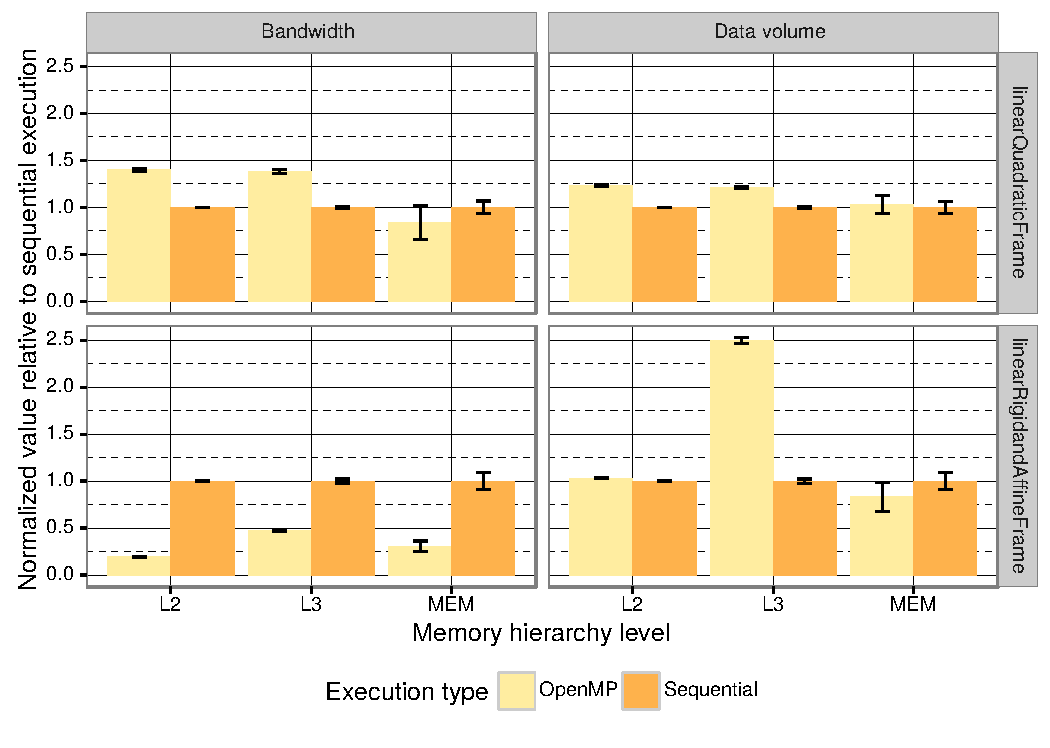
\includegraphics[width=\textwidth]{SOFA_perfctr.pdf}
    \caption[SOFA likwid results]{Differences of bandwidth and data volume, from L2 cache to main memory, between sequential and parallel execution of \gls{SOFA} on two different simulation scenes.
        \\
        For both bandwidth and data volume, the value is normalized to the mean value of the corresponding sequential executions.
        \\
        For bandwidth, higher is better while for data volume lower is better.
    }
    \label{fig:SOFA-perfctr}
\end{figure}

\fig{SOFA-perfctr} shows the bandwidth (left side) and the data volume (right sides) for the two functions (\emph{linearQuadraticFrame} above, \emph{linearRigidAndAffineFrame} below) from \texttt{L2} cache to the main memory.
Each point represents the mean of $60$ runs and the error bars represents the standard error.
To make the plot more readable, we have normalized each value by dividing it by the value for the corresponding sequential run, thus these plots show the evolution of the bandwidth and data volume when we use the \gls{OpenMP} version of\gls{SOFA}.

We can see that for the first scene, both the bandwidth and data volume increases by a factor of $1.5$ in the cache and stays comparable in the main memory when we use the parallel version.
This means that the thread are either sharing efficiently data or at least working on data different enough to not step on each other foots.
At the opposite for the second scene, the bandwidth drops down at each level and the data volume stays still except at the \texttt{L3} level where it increases by a factor $2.5$.
It is important to note that the \texttt{L3} cache is the only shared cache which means that a considerable amount of data is invalidated in \texttt{L2}, in other words, several threads are writing the same data, invalidating each other private cache and requiring the coherency protocol to interfere.
This behavior is called false sharing and is a well known performance issue.

At this point we can say that false sharing occurs on this precise function, yet we do not know on which data structure.
We could dig onto the code and try to understand the memory access pattern of each data structure to see where the false sharing does occurs.
By looking at \gls{SOFA}'s code, we can see that the main difference between the two version of the function is that for \texttt{linearRigidAndAffineFrame} there is one more loop in the computation.
Still this code manipulate several data through many indirections, therefore determining on which data the false sharing is happening could be extremely slow.
Furthermore this approach is not generic at all, and once we have done it for one particular function, we would have to redo the same analysis and optimization for each potential hotspot.

Furthermore as we have seen with the runtime ratio, this particular false sharing issue only represent a small part of the execution, therefore a more generic approach would be welcome.

From that point it seems clear that \gls{SOFA} is having memory performance issues, yet we need a generic tools to analyze its performances from the memory point of view.
Such tool should be able to show the memory access patterns of each thread over the different data structures and point us through patterns that are (or can be) inefficient.

% vim: et si sta lbr  sw=4 ts=4 spelllang=en_us
